%-------------------------------------------------------------------------------
\chapter{Anticipation using approximate models}
\label{ch.mpc}
\acresetall
%-------------------------------------------------------------------------------

We have indicated in \cref{sec.balance_general}, that awareness of the future
is crucial for balance preservation in a general setting. It is, however, often
sufficient to look into the future for a limited time horizon. This can be
achieved with \ac{MPC} \cite{Rawlings2009mpc, Maciejowski2002mpc}, which is the
subject of the present chapter. The discussion begins with a brief overview of
\ac{MPC} in \cref{sec.mpc_overview}, which is followed by
\cref{sec.approx_models_discret,sec.approx_models_capturability}, where we
discretize the continuous-time approximate models constructed in
\cref{sec.linear_approx_models} and derive capturability constraints for them.
In the last two \cref{sec.mmpc,sec.sampling_interval} we introduce \ac{MMPC}
and discuss the choice of duration of sampling intervals.



%%%%%%%%%%%%%%%%%%%%%%%%%%%%%%%%%%%%%%%%%%%%%%%%%%%%%%%%%%%%%%%%%%%%%%%%%%%%%%%%
%%%%%%%%%%%%%%%%%%%%%%%%%%%%%%%%%%%%%%%%%%%%%%%%%%%%%%%%%%%%%%%%%%%%%%%%%%%%%%%%
%%%%%%%%%%%%%%%%%%%%%%%%%%%%%%%%%%%%%%%%%%%%%%%%%%%%%%%%%%%%%%%%%%%%%%%%%%%%%%%%
\section{Overview of Model Predictive Control}\label{sec.mpc_overview}

The name of the \acf{MPC} paradigm stresses two of its important components: a
model of the system, and a prediction of its evolution. In this thesis, we
employ linear discrete-time models of the form
%
\begin{subequations}
\begin{empheq}[left=\empheqlbrace]{align}
    &\V{x}_{k+1} = \M{A}_k \V{x}_k + \M{B}_k \V{u}_k, \quad k \in \{0, ..., N-1\}
    \label{eq.discrete_linear_system_dynamics}
    \\
    &\V{x}_{k+1} \in \SET{X}_{k+1},
    \\
    &\V{u}_k \in \SET{U}_k.
\end{empheq}
\end{subequations}
%
The prediction is used to choose a sequence of $N$ control inputs $(\V{u}_{0},
..., \V{u}_{N-1})$, such that the future states $(\V{x}_{1}, ..., \V{x}_{N})$
comply with the constraints of the model. In some cases, the constraints
uniquely determine the future evolution of the model and controls can be found
analytically. In general, however, a selection criterion for controls is
needed, which is typically expressed as a least-squares objective, for example,
%
\begin{equation}
    \begin{aligned}
        \MINIMIZE{\V{u}_{0}, ..., \V{u}_{N-1}}
        &
        \sum_{k=0}^{N-1}
        \left(
            \NORME{\M{\Gamma}_{\V{u}} \V{u}_{k}}^2
            +
            \NORME{\M{\Gamma}_{\V{x}} \V{x}_{k+1}}^2
        \right)
        ,
        \\
    \end{aligned}
\end{equation}
%
where $\M{\Gamma}_u$ and $\M{\Gamma}_x$ are weighting matrices. Given the
constraints of the model and a selection criterion for controls we express an
\ac{MPC} problem as a \ac{QP} \cite{Nocedal2006numopt, Boyd2004conopt}, which
can be solved with off-the-shelf software, for example, \sn{qpOASES}
\cite{Ferreau2014mpc}.

%
\begin{figure}[ht]
    \centering{%
    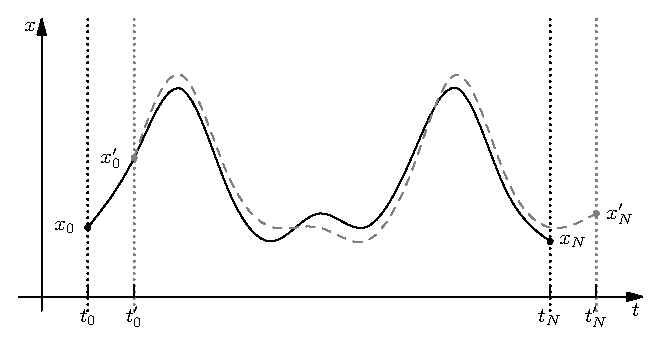
\includegraphics{mpc_idea.eps}}
    \caption[Shift of the preview horizon in Model Predictive Control.]{
        Shift of the preview horizon in \ac{MPC}. Trajectory of state $x$
        previewed starting from time $t_0$ is recomputed at time
        $t_0^{\prime}$. Length of the preview horizon is $H = t_N - t_0 =
        \sum_{k=0}^{N-1} T_k$, where $N$ is the number of sampling intervals
        and $T_k$ is the duration of $k$-th interval.
    }
    \label{fig.mpc_idea}
\end{figure}
%

The key feature of \ac{MPC} is that the control problem is resolved
periodically in order to realize state feedback. Hence, not all $N$ control
inputs are applied, instead, the \ac{MPC} problem is updated and resolved after
a short time, usually one sampling interval, as illustrated in
\cref{fig.mpc_idea}.


%%%%%%%%%%%%%%%%%%%%%%%%%%%%%%%%%%%%%%%%%%%%%%%%%%%%%%%%%%%%%%%%%%%%%%%%%%%%%%%%
%%%%%%%%%%%%%%%%%%%%%%%%%%%%%%%%%%%%%%%%%%%%%%%%%%%%%%%%%%%%%%%%%%%%%%%%%%%%%%%%
%%%%%%%%%%%%%%%%%%%%%%%%%%%%%%%%%%%%%%%%%%%%%%%%%%%%%%%%%%%%%%%%%%%%%%%%%%%%%%%%
\section{Discretization of approximate models}\label{sec.approx_models_discret}

Standard approaches to \ac{MPC} rely on discrete-time models. For this reason,
we discretize the linear continuous-time models constructed in
\cref{sec.linear_approx_models} with the help of \sn{Maxima} \ac{CAS}
\cite{MAXIMAsite}. Discretization is performed in the standard way with
\tn{zero-order hold} for controls, \IE, the discrete-time models have constant
controls during a sampling interval \cite[Chapter~1]{BaoCang2010mpc}.


In all considered discrete-time models, $k$ denotes the index of a sampling
interval and $T_k$ is the duration of this interval.



%%%%%%%%%%%%%%%%%%%%%%%%%%%%%%%%%%%%%%%%%%%%%%%%%%%%%%%%%%%%%%%%%%%%%%%%%%%%%%%%
\subsection{Momenta-based model}\label{sec.momenta_model_discret}

Discretization of \nameref{model.CMB} model yields
%
\begin{model}{MB}{}
\begin{subequations}\label{eq.discrete_momenta_model}
\begin{empheq}[left=\empheqlbrace]{align}
    &
        \V{x}_{k+1}
        =
        \underbrace{
            \begin{bmatrix}
                \V{I}             & T_k \V{I}                           & \V{0}\\
                \V{0}             & \V{I}                               & \V{0}\\
                T_k \tildeM{A}  & \frac{T_k^2}{2} \tildeM{A}    & \V{I}
            \end{bmatrix}
        }_{\M{A}_k}
        \V{x}_{k}
        +
        \sum_{i=1}^{M_k}
        \underbrace{
            \begin{bmatrix}
                \frac{T^2_k}{2} \Ixy                                                & \V{0}\\
                T_k \Ixy                                                            & \V{0}\\
                T_k\tildeM{B}_{k,i} + \frac{T^3_k}{6}\tildeM{A} \Ixy                & T_k \Ixy
            \end{bmatrix}
        }_{\M{B}_{k,i}}
        \wrench_{k,i}
        +
        \underbrace{
            \begin{bmatrix}
                \frac{T^2_k}{2} \tildeV{b} \\
                T_k \tildeV{b} \\
                \frac{T^3_k}{6} \tildeM{A} \tildeV{b}
            \end{bmatrix}
        }_{\V{b}},
        \label{eq.discrete_momenta_model.dynamics}
        \\
    & \force_{k,i} = \M{V}_{k,i} \V{\lambda}_{k,i},
      \\
    &
        \sum_{i=1}^{M_k} \forceC_{k,i}^z = - m g^z
        ,
        \\
    &
        \objA_{\moment,k,i}
        \begin{bmatrix}
            \V{\lambda}_{k,i}\\
            \moment_{k,i}
        \end{bmatrix}
        \ge
        \ubarV{\objb}_{\moment,k,i}
        ,
        \\
    & \V{\lambda}_{k,i} \ge \V{0},
        \label{eq.discrete_momenta_model.friction}\\
    & \mbox{proxy constraints},
        \label{eq.discrete_momenta_model.fixedcontact}
\end{empheq}
\end{subequations}
\end{model}
%
where the state vector $\V{x}$ and matrices $\tildeM{A}$, $\tildeV{b}$ are
defined as in \cref{sec.model_momenta}, contact wrench $\wrench_{k,i} =
(\force_{k,i}, \moment_{k,i})$ is constant during $T_k$, $M_k$ is the number of
contacts during the $k$-th interval, and $\tildeM{B}_{k,i}$ in contrast with
$\tildeM{B}_{i}$ used in continuous-time \nameref{model.CMB} model allows for
different positions of contacts $\contact_{k,i}$ during different intervals
%
\begin{equation}
    \tildeM{B}_{k,i}
    =
    \begin{bmatrix}
        0                       & - (\contactC_{k,i}^z - {c}^z)   & \contactC_{k,i}^y\\
        \contactC_{k,i}^z - {c}^z     & 0                         & - \contactC_{k,i}^x
    \end{bmatrix}.
\end{equation}
%



%%%%%%%%%%%%%%%%%%%%%%%%%%%%%%%%%%%%%%%%%%%%%%%%%%%%%%%%%%%%%%%%%%%%%%%%%%%%%%%%
\subsection{Point-mass models with planar CoM motion}\label{sec.point_mass_planar_discret}

In the following subsections we discretize \nameref{model.CPPMJ} and
\nameref{model.CPPMdZ} models presented in \cref{sec.point_mass_planar}. For
simplicity we assume that
%
\begin{description}
    \item[\ass{ass.constant_ext_wrench}] the external wrench $(\forceext,
        \momentext)$ and orientation of the gravity $\V{g}$ do not change
        within the preview horizon;

    \item[\ass{ass.constant_foot_height}] the vertical position of contact
        points $\contactC^z$ is constant.
\end{description}
%
It is possible to generalize the derivations to situations, when these
assumptions do not hold. This, however, would require a larger number of
constraints on the \ac{CoP} positions.



%%%%%%%%%%%%%%%%%%%%%%%%%%%%%%%%%%%%%%%%%%%%%%%%%%%%%%%%%%%
\subsubsection{Model controlled with the CoM jerk}\label{sec.point_mass_planar_discret_jerk}

Discretization of \nameref{model.CPPMJ} model yields
%
\begin{model}{PPMJ}{Planar Point-Mass controlled with \acs{CoM} Jerk}
\begin{subequations}\label{eq.ppmj}
    \begin{empheq}[left=\empheqlbrace]{align}
        &
            \V{x}_{k+1}
            =
            \begin{bmatrix}
                \tildeM{A}_k  & \M{0} \\
                \M{0}   & \tildeM{A}_k  \\
            \end{bmatrix}
            \V{x}_k
            +
            \begin{bmatrix}
                \tildeV{B}_k & \V{0}\\
                \V{0}  & \tildeV{B}_k \\
            \end{bmatrix}
            \dddotV{c}_k^{xy}
            ,
            \\
        &
            \cop_{k+1}
            =
            \begin{bmatrix}
                \tildeM{D} & \M{0}\\
                \M{0} & \tildeM{D}\\
            \end{bmatrix}
            \V{x}_{k+1}
            +
            \FUNC{Z}(\zeta, \V{g}, \forceext, \momentext)
            ,
            \label{eq.ppmj.cop}
            \\[2mm]
        &
            \cop_{k+1} \in \SET{S}(\contact_{k+1,1}^{xy}, ... ,\contact_{k+1,M_s}^{xy})
            ,
    \end{empheq}
\end{subequations}
\end{model}
%
where $k \in \{0, ..., N-1\}$,
$
\V{x}_k =
(
    \C{c}^x_k,
    \dotC{c}^x_k,
    \ddotC{c}^x_k,
    \C{c}^y_k,
    \dotC{c}^y_k,
    \ddotC{c}^y_k
)
$,
%
\begin{equation}
    \tildeM{A}_k =
    \begin{bmatrix}
        1       & T_k   & T_k^2/2\\
        0       & 1     & T_k    \\
        0       & 0     & 1      \\
    \end{bmatrix}
    ,
    \quad
    \tildeM{B}_k =
    \begin{bmatrix}
        T_k^3/6 \\
        T_k^2/2 \\
        T_k     \\
    \end{bmatrix}
    ,
    \\
    \quad
    \tildeM{D}
    =
    \begin{bmatrix}
        1 & 0 &  - \zeta
    \end{bmatrix}
    ,
    \quad
    \zeta
    =
    \frac{m (c^z - \contactC^z)}{- m \C{g}^z - \forceextC^z}
    .
\end{equation}
%
\begin{equation}
    \FUNC{Z}(\zeta, \V{g}, \forceext, \momentext)
    =
    \zeta
    \left(
        \V{g}^{xy}
        +
        \frac{\forceext^{xy}}{m}
    \right)
    +
    \frac{1}{- m \C{g}^z - \forceextC^z}
    \begin{bmatrix}
        - \momentextC^y\\
        \momentextC^x\\
    \end{bmatrix}
\end{equation}
%


Note that, if one of the parameters in \cref{eq.ppmj.cop} changes at the
boundary between the $k$-th and $k+1$ sampling intervals, there is a
discontinuity in the \ac{CoP} position at this instant. Hence, if, for example,
the external force $\forceext$ changes at this instant, the number of
constraints on the \ac{CoP} position must be doubled. For the same reason it is
necessary to impose the \ac{CoP} constraints twice for each sampling interval
in the case of the second order model based on a double integrator and
controlled with the \ac{CoM} acceleration. In order to avoid this complication
we introduced \cref{ass.constant_ext_wrench,ass.constant_foot_height}.


Satisfaction of the constraints on $\cop_k$ and $\cop_{k+1}$ in the models
controlled by the \ac{CoM} acceleration or jerk does not guarantee their
satisfaction during the $k$-th sampling interval. In order to illustrate this we
consider the $k$-th sampling interval of the system controlled by the \ac{CoM}
jerk. Let $\V{x}_k$ be an initial state, $\dddotV{c}_k^{xy}$ -- the constant
jerk applied during $T_k$, $\V{x}_t$ -- the state of the system at some $t \in
[0, T_k]$. Position of the \ac{CoP} during the sampling interval can be found
as
%
\begin{equation}
    \copC^\alpha_t
    =
    \tildeM{D}_k
    \begin{bmatrix}
        \C{c}^\alpha_t\\
        \dotC{c}^\alpha_t\\
        \ddotC{c}^\alpha_t
    \end{bmatrix}
    =
    \tildeM{D}_k
    \left(
        \tildeM{A}_t
        \begin{bmatrix}
            \C{c}^\alpha_k\\
            \dotC{c}^\alpha_k\\
            \ddotC{c}^\alpha_k
        \end{bmatrix}
        +
        \tildeM{B}_t
        \dddotC{c}^{\alpha}_k
    \right)
    ,
\end{equation}
%
where $\alpha \in \{x,y\}$, $(\forceext[k,], \momentext[k,]) = \V{0}$ for
simplicity, and
%
\begin{equation}
    \tildeM{A}_t =
    \begin{bmatrix}
        1       & t   & t^2/2\\
        0       & 1     & t    \\
        0       & 0     & 1      \\
    \end{bmatrix}
    ,
    \quad
    \tildeM{B}_t =
    \begin{bmatrix}
        t^3/6 \\
        t^2/2 \\
        t       \\
    \end{bmatrix}
    .
\end{equation}
%
Hence, the \ac{CoP} position at time $t$ depends cubically on time $t$:
%
\begin{equation}\label{eq.cop_polynomial}
    \copC_t^\alpha
    =
    \frac{\dddotC{c}_k^\alpha}{6} t^3
    +
    \frac{\ddotC{c}_k^\alpha}{2} t^2
    +
    \left(
        \dotC{c}_k^\alpha
        -
        \dddotC{c}_k^\alpha \zeta_k
    \right)
    t
    -
    \ddotC{c}_k^\alpha \zeta_k
    +
    \C{c}_k^\alpha.
\end{equation}
%
Similarly, this dependence is quadratic in the case of a second order model
controlled by the \ac{CoM} acceleration. Therefore, satisfaction of the
\ac{CoP} constraints at time $0$ and $T_k$, as is usually enforced by \ac{MPC}
schemes, does not guarantee their satisfaction at $t \in (0, T_k)$. The systems
controlled by the \ac{CoP} position or its velocity are not subject to this
problem. This problem, however, is typically not critical, since the support
areas are intentionally shrunk due to the addition of safety margins
\cite{Wieber2015handbook}. The size of these margins can be estimated by
computing maxima of the polynomial \cref{eq.cop_polynomial}.



%%%%%%%%%%%%%%%%%%%%%%%%%%%%%%%%%%%%%%%%%%%%%%%%%%%%%%%%%%%
\subsubsection{System controlled with the CoP velocity}\label{sec.point_mass_planar_discret_dcop}

\begin{figure}[ht]
    \begin{minipage}[t]{0.45\textwidth}
        \centering{%
        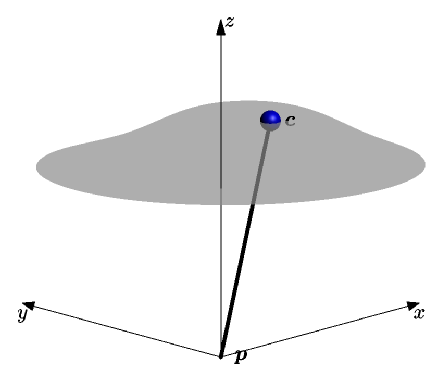
\includegraphics{inverted_pendulum.eps}}
        \caption{Inverted pendulum with a mass $\V{c}$ constrained to a plane.}
        \label{fig.inverted_pendulum1}
    \end{minipage}
    \hfill
    \begin{minipage}[t]{0.45\textwidth}
        \centering{%
        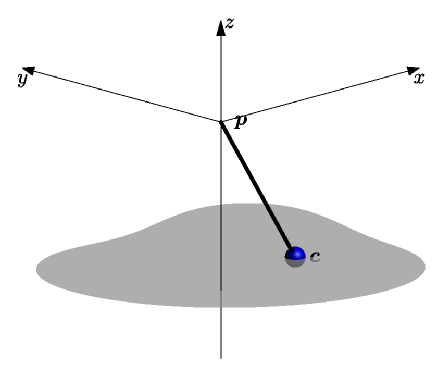
\includegraphics{pendulum.eps}}
        \caption{Pendulum with a mass $\V{c}$ constrained to a plane.}
        \label{fig.pendulum1}
    \end{minipage}
\end{figure}


Discretized version of \nameref{model.CPPMdZ} is
%
\begin{model}{PPMdZ}{Planar Point-Mass controlled with $\dot{\cop}$}
\begin{subequations}
    \begin{empheq}[left=\empheqlbrace]{align}
        &
            \V{x}_{k+1}
            =
            \begin{bmatrix}
                \tildeM{A}_k  & \M{0} \\
                \M{0}   & \tildeM{A}_k  \\
            \end{bmatrix}
            \V{x}_k
            +
            \begin{bmatrix}
                \tildeV{B}_k & \V{0}\\
                \V{0}  & \tildeV{B}_k \\
            \end{bmatrix}
            \dot{\cop}_k
            ,
            \\
        &
            \cop_{k+1}
            =
            \begin{bmatrix}
                \tildeM{D} & \M{0}\\
                \M{0} & \tildeM{D}\\
            \end{bmatrix}
            \V{x}_{k+1}
            +
            \FUNC{Z}(\zeta, \V{g}, \forceext, \momentext)
            ,
            \\[2mm]
        &
            \cop_{k+1} \in \SET{S}(\contact_{k+1,1}^{xy}, ... ,\contact_{k+1,M_s}^{xy})
            ,
    \end{empheq}
\end{subequations}
\end{model}
%
where all terms are defined as in \nameref{model.PPMJ} model, except matrices
$\tildeM{A}_k$ and $\tildeV{B}_k$, which differ depending on the sign of
$\zeta$
%
\begin{equation}
    \zeta
    =
    \frac{m (c^z - \contactC^z)}{- m \C{g}^z - \forceextC^z}.
\end{equation}
%
Note that we already have $\zeta \ne 0$ due to \cref{ass.nonzero_com_height}.
%
\begin{itemize}
    \item The variable $\zeta$ is negative, when $c^z - \contactC^z > 0$ and $-
        m \C{g}^z < \forceextC^z$, or $c^z - \contactC^z < 0$ and $- m \C{g}^z
        > \forceextC^z$. This is possible in two cases: ({\bf i}) the \ac{CoM}
        is below the support surface and $\forceextC^z$ does not cancel the
        gravity, ({\bf ii}) the \ac{CoM} is above the support surface and
        $\forceextC^z$ cancels the gravity. In any case, the robot is hanging
        and its dynamics resembles dynamics of a standard pendulum shown in
        \cref{fig.pendulum1}. We are not aware of publications, where this
        version of the model was employed, but it may be useful in some
        settings, for example, to realize locomotion on monkey bars as in
        \cite{Dai2014humanoids}, which relies on a nonlinear model. So,
        whenever $\zeta < 0$, the matrices are defined as
        \vspace{-\parskip}\par
        %
        {
        \small
        \begin{equation}
            \label{eq.ppmdz_matrices1}
            \tildeM{A}_k
            =
            \begin{bmatrix}
                1   &   \sin \left(\frac{T_k}{\sqrt{ \NORM{\zeta}}}\right) \sqrt{ \NORM{\zeta}}  &   \zeta\cos \left(\frac{T_k}{\sqrt{ \NORM{\zeta}}}\right) - \zeta \\
                0   &   \cos \left(\frac{T_k}{\sqrt{ \NORM{\zeta}}}\right)   &   \sin \left(\frac{T_k}{\sqrt{ \NORM{\zeta}}}\right) \sqrt{ \NORM{\zeta}} \\
                0   &   -\frac{1}{\sqrt{\NORM{\zeta}}} \sin \left(\frac{T_k}{\sqrt{ \NORM{\zeta}}}\right)   &   \cos \left(\frac{T_k}{\sqrt{ \NORM{\zeta}}}\right) \\
            \end{bmatrix}
            ,
            \enspace
            \tildeM{B}_k
            =
            \begin{bmatrix}
                T_k - \sin \left(\frac{T_k}{\sqrt{ \NORM{\zeta}}}\right) \sqrt{ \NORM{\zeta}} \\
                1 - \cos \left(\frac{T_k}{\sqrt{ \NORM{\zeta}}}\right) \\
                \frac{1}{\sqrt{\NORM{\zeta}}} \sin \left(\frac{T_k}{\sqrt{ \NORM{\zeta}}}\right)\\
            \end{bmatrix}
            .
        \end{equation}
        }
        %

    \item In the case of positive $\zeta$, which corresponds to \ac{LIPM}
        (\cref{fig.inverted_pendulum1}), the matrices have the following form
        %
        \begin{equation}
            \label{eq.ppmdz_matrices2}
            \tildeM{A}_k
            =
            \begin{bmatrix}
                1   &   \sinh \left(\frac{T_k}{\sqrt{\zeta}}\right) \sqrt{\zeta} &   \zeta\cosh \left(\frac{T_k}{\sqrt{\zeta}}\right) - \zeta \\
                0   &   \cosh \left(\frac{T_k}{\sqrt{\zeta}}\right)  &   \sinh \left(\frac{T_k}{\sqrt{\zeta}}\right) \sqrt{\zeta} \\
                0   &   \frac{1}{\sqrt{\zeta}}\sinh \left(\frac{T_k}{\sqrt{\zeta}}\right)     &   \cosh \left(\frac{T_k}{\sqrt{\zeta}}\right)\\
            \end{bmatrix}
            ,
            \quad
            \tildeM{B}_k
            =
            \begin{bmatrix}
                T_k - \sinh \left(\frac{T_k}{\sqrt{\zeta}}\right) \sqrt{\zeta} \\
                1 - \cosh \left(\frac{T_k}{\sqrt{\zeta}}\right) \\
                - \frac{1}{\sqrt{\zeta}} \sinh \left(\frac{T_k}{\sqrt{\zeta}}\right)
            \end{bmatrix}
            .
        \end{equation}
        %
        Note that substitution of negative $\zeta$ in the obtained matrices
        yields \cref{eq.ppmdz_matrices1}, hence, they are expressed in
        \cref{eq.ppmdz_matrices2} in a more general form.
\end{itemize}
%




%%%%%%%%%%%%%%%%%%%%%%%%%%%%%%%%%%%%%%%%%%%%%%%%%%%%%%%%%%%%%%%%%%%%%%%%%%%%%%%%
\subsection{Point-mass model with nonplanar CoM motion}

Discretization of \nameref{model.CNPM} model presented in
\cref{sec.point_mass_nonplanar} is trivial as in the case of
\nameref{model.CPPMJ} model with planar \ac{CoM} motion (see
\cref{sec.point_mass_planar_discret_jerk}).



%%%%%%%%%%%%%%%%%%%%%%%%%%%%%%%%%%%%%%%%%%%%%%%%%%%%%%%%%%%%%%%%%%%%%%%%%%%%%%%%
\subsection{Variation of discrete-time models with time}\label{sec.discret_variation}

One can observe that state transition matrices, control matrices, and
constraints in discrete-time models can be chosen differently depending on the
sampling interval $k$. Hence, some parameters of the models, which were assumed
to be constant in continuous-time case, can vary in discrete-time case if their
changes are known in advance and synchronized with the boundaries of sampling
intervals. For example,
%
\begin{itemize}
    \item The number and positions of contacts can be changed in momenta-based
        model as hinted in \cref{sec.momenta_model_discret}. Therefore, this
        model can be used to realize locomotion \cite{Nagasaka2012,
        Audren2014iros}.

    \item Variation of the discrete-time models with planar \ac{CoM} motion is
        used to change foot contacts and orientations of the feet without
        compromising linearity \cite{Herdt2010auro},
        \cref{sec.mpc_foot_positions}.

    \item The point-mass model with nonplanar \ac{CoM} motion can be utilized
        for walking on an uneven terrain, if height of the contact surface
        $\contactC^z_k$ as well as its orientation are changed appropriately
        \cite{Brasseur2015humanoids}.
\end{itemize}
%


Variation of the discrete-time models is typically realized with the help of
external routines with respect to \ac{MPC}. For example, a preliminary \ac{MPC}
problem is solved in \cite[Chapter~2]{Herdt2012thesis} to determine
orientations of the foot contacts. In the same work, a \ac{FSM} is used to set
durations and alternation of left and right foot contacts during a regular
walk. Though durations of the contacts are usually decided externally when
approximate models are employed, in some settings this can be partially avoided
with the help of motion anticipation and task prioritization as described in
\cref{sec.optional_force} and \cite{Sherikov2015humanoids}.



%%%%%%%%%%%%%%%%%%%%%%%%%%%%%%%%%%%%%%%%%%%%%%%%%%%%%%%%%%%%%%%%%%%%%%%%%%%%%%%%
%%%%%%%%%%%%%%%%%%%%%%%%%%%%%%%%%%%%%%%%%%%%%%%%%%%%%%%%%%%%%%%%%%%%%%%%%%%%%%%%
%%%%%%%%%%%%%%%%%%%%%%%%%%%%%%%%%%%%%%%%%%%%%%%%%%%%%%%%%%%%%%%%%%%%%%%%%%%%%%%%
\section{Capturability constraints}\label{sec.approx_models_capturability}

We claimed in \cref{sec.balance_general} that balance is maintained as long as
it is possible to stop the robot, \IE, capture it, without violation of the
system constraints. A capturability constraint on the final state-control pair
$(\V{x}_N, \V{u}_{N+1})$ formalizes conditions under which the robot can be
stopped. In this regard the capturability constraint is similar to the so
called \tn{terminal constraint}, which is employed in \tn{dual-mode} \ac{MPC}
\cite{Mayne2000automatica}, \cite[Chapter~6]{Rossiter2003mpc}. In this version
of \ac{MPC} a terminal constraint is imposed at the end of the preview horizon
to make sure that the system reaches some \tn{terminal set}, where a simple
local controller can stabilize the system. Here we take a similar approach, but
we want a local controller to drive the system to \tn{any} of its statically
balanced states instead of \tn{a given desired} state. Our approach is
conceptually similar to constraining the final state-control pair to a
\tn{terminal feasible invariant set} as suggested in
\cite{Schouwenaars2006thesis}.


There are several conceptual questions regarding capturability constraints,
which we would like to address before going into details of construction of
these constraints for particular models:
%
\begin{itemize}
    \item Shouldn't we aim for stability rather than capturability? So far we
        cannot give a decisive answer. Capturability is in general less
        restrictive as indicated above. On the other hand, closed loop behavior
        of an \ac{MPC} with capturability constraints may be worse, for
        example, due to different statically balanced states being chosen on
        different control iterations.

    \item Why many applications of \ac{MPC} for balance preservation are
        successful without capturability constraints \cite{Herdt2010auro,
        Kajita2003icra} and what kind of improvements such constraints can
        bring? The answer to the first part of the question lies in the fact
        that a finite preview horizon \tn{approximates} an infinite preview
        horizon, which, in turn, guarantees viability, \IE, that the robot will
        not fall \cite{Wieber2008iros}. A capturability constraint, on the
        other hand, \tn{guarantees} capturability, \IE, the ability to stop,
        even with a finite preview horizon. Hence, an \ac{MPC} problem with
        capturability constraint is more reliable in balance preservation and
        does not need the preview horizon to be as long as in the case without
        such constraint.

    \item What is the impact of a capturability constraint on feasibility of
        the underlying optimization problem? A capturability constraint, as
        well as any other hard constraint, may cause infeasibility
        \cite[Chapter~8]{Rossiter2003mpc}, which means that the chosen model of
        the robot cannot be stopped within the chosen preview horizon. This
        infeasibility is equivalent to a conflict between tasks in whole body
        motion control reviewed in \cref{sec.wbm_control} and, thus, can be
        addressed with the same numerical tools, which are discussed in
        \cref{ch.optimization}.
\end{itemize}
%


In the following subsections we construct capturability constraints for the
approximate models introduced in \cref{sec.linear_approx_models} and
discretized in \cref{sec.approx_models_discret}. In all cases we derive
constraints assuming that
%
\begin{description}
    \item[\ass{ass.timeinvariant}] The model is time-invariant, starting from
        the end of the preview horizon, which implies, in particular, that the
        number and positions of the contacts do not change. Note that our
        capturability constraints ensure recursive feasibility of
        time-invariant systems in the same way as the usual terminal
        constraints \cite{Mayne2000automatica}.
\end{description}
%
It is also presumed that the system constraints are imposed on the final
state-control pair in addition to the derived capturability constraints.



%%%%%%%%%%%%%%%%%%%%%%%%%%%%%%%%%%%%%%%%%%%%%%%%%%%%%%%%%%%%%%%%%%%%%%%%%%%%%%%%
\subsection{Momenta-based model}\label{sec.momenta_model_capturability}
In its simplest form a capturability constraint imposes that the robot is in a
statically balanced state. A statically balanced state must necessarily be a
part of a fixed point, \IE, such state-control pair $(\V{x}_k, \V{u}_k)$ that
\cite[Chapter~8]{Scheinerman1996ids}
%
\begin{equation}
    \V{x}_k = \M{A}_k \V{x}_k + \M{B}_k \V{u}_k.
\end{equation}
%
In the case of momenta-based (\nameref{model.MB}) model, this condition results
in the following constraints, where indices of state and control variables are
omitted for simplicity:
%
\begin{itemize}
    \item $\V{\LM}^{xy} = \V{0}$ -- no linear momentum in the $x$-$y$ plane,
        \IE, the \ac{CoM} velocity is zero $\dotV{c}^{xy} = \V{0}$;

    \item $m \V{g}^{xy} + \sum_{i=1}^{M} \force_i^{xy} = \V{0}$ -- no forces in
        the $x$-$y$ plane, \IE, the \ac{CoM} acceleration is zero
        $\ddotV{c}^{xy} = \V{0}$;

    \item the rate of change of the angular momentum about the $x$ and $y$ axes
        is also zero:
        \begin{equation}
            \begin{aligned}
                \dotV[c]{\AM}^{xy}
                &=
                \begin{bmatrix}
                        \hatC{\LM}^y \C{g}^z
                        +
                        \sum_{i=1}^{M}
                        \left(
                            \forceC^z_i \contactC_i^y
                            +
                            \Ix \moment_i
                            -
                            \forceC^y_i (\contactC^z_i - \C{c}^z)
                        \right)
                    \\
                        -\hatC{\LM}^x \C{g}^z
                        +
                        \sum_{i=1}^{M}
                        \left(
                            -\forceC^z_i \contactC_i^x
                            +
                            \Iy \moment_i
                            +
                            \forceC^x_i (\contactC^z_i - \C{c}^z)
                        \right)
                \end{bmatrix}
                \\
                &=
                \begin{bmatrix}
                        \hatC{\LM}^y \C{g}^z
                        -
                        m \C{c}^z \C{g}^y
                        +
                        \sum_{i=1}^{M}
                        \left(
                            \forceC^z_i \contactC_i^y
                            +
                            \Ix \moment_i
                            -
                            \forceC^y_i \contactC^z_i
                        \right)
                    \\
                        -\hatC{\LM}^x \C{g}^z
                        +
                        m \C{c}^z \C{g}^x
                        +
                        \sum_{i=1}^{M}
                        \left(
                            - \forceC^z_i \contactC_i^x
                            +
                            \Iy \moment_i
                            +
                            \forceC^x_i \contactC^z_i
                        \right)
                \end{bmatrix}
                =
                \V{0}.
            \end{aligned}
        \end{equation}
\end{itemize}
%
Note that the fixed points of the approximate system include states with
non-zero angular momentum $\V[c]{\AM}^{xy} \neq \V{0}$, even though the real
system cannot store angular momentum \cite{Stephens2010iros}. Consequently, a
fixed point of this approximate model does not always correspond to a fixed
point of the whole body model and does not imply that the latter is captured.
We alleviate this issue by imposing that $\V[c]{\AM}^{xy}$ is zero as well.
Furthermore, provided that $m \V{g}^{xy} + \sum_{i=1}^{M} \force_i^{xy} =
\V{0}$ holds, we can also determine $\dotC[c]{\AM}^{z}$ using the equation
\cref{eq.component_wise_momenta} and constrain it:
%
\begin{equation}
    \begin{aligned}
        \dotC[c]{\AM}^z
        &=
        \sum_{i=1}^M
        \left(
            \begin{bmatrix}
                - (\contactC_i^y - {c}^y) & \contactC_i^x - {c}^x       & 0
            \end{bmatrix}
            \force_i
            +
            \Iz
            \moment_i
        \right)
        \\
        & =
        \sum_{i=1}^M
        \left(
            \contactC_i^x
            \forceC_i^y
            -
            \contactC_i^y
            \forceC_i^x
            +
            \Iz
            \moment_i
        \right)
        +
        \hatC{\LM}^x
        \C{g}^y
        -
        \hatC{\LM}^y
        \C{g}^x
        =
        0
        ,
    \end{aligned}
\end{equation}
%
even though $\dotC[c]{\AM}^z$ depends nonlinearly on the state and control
variables in general.


Thus, the complete capturability constraint is defined as
%
\begin{subequations}
    \label{eq.capture_momenta_model}
    \begin{empheq}[left=\empheqlbrace]{alignat=2}
        &\V{\LM}^{xy}
        &&= \V{0},
        \\
        &\V[c]{\AM}^{xy}
        &&= \V{0},
        \\
        &\dotV{\LM}^{xy}
        &&= m \V{g}^{xy} + \sum_{i=1}^{M} \force_i^{xy} = \V{0},
        \\
        &
        \dotV[c]{\AM}
        &&=
        -
        \V{g}
        \CROSS
        \begin{bmatrix}
            \hatV{\LM}^{xy}\\
            m \C{c}^z
        \end{bmatrix}
        +
        \sum_{i=1}^{M}
        \left(
            \contact_i
            \CROSS
            \force_i
            +
            \moment_i
        \right)
        =
        \V{0}
        .
    \end{empheq}
\end{subequations}
%
Note that the capturability constraint imposed in \cite{Sherikov2015humanoids}
for the same model is not entirely correct.



%%%%%%%%%%%%%%%%%%%%%%%%%%%%%%%%%%%%%%%%%%%%%%%%%%%%%%%%%%%%%%%%%%%%%%%%%%%%%%%%
\subsection{Point-mass models with planar CoM motion}\label{sec.point_mass_planar_capturability}

In the present section we construct capturability constraints for the two third
order point-mass models introduced in \cref{sec.point_mass_planar} and
discretized in \cref{sec.point_mass_planar_discret}. We approach the derivation
of these constraints using the idea of dual-mode \ac{MPC} instead of
identification of fixed points as in the previous case of the momenta-based
model. To be more precise, we use capturability constraints to specify a set of
states, starting from which the system can converge to a statically balanced
state with the help of a simple linear feedback controller. Strictly speaking,
\tn{convergence} to a statically balanced state contradicts with our definition
of capturability given in \cref{ch.balance}, since this definition requires
that the system reaches a statically balanced state in \tn{finite} time.
However, we consider this contradiction to be insignificant.


We construct linear feedback controllers in such a way, that they maintain a
constant position of the \ac{CoP}. This implies that constraints on this
position will not be violated in the future. Though the controllers are
supposed to be discrete-time, we consider their continuous-time counterparts as
well to emphasize relations and differences between variants of the model with
different control variables.


In order to simplify presentation, we exploit the fact, that the state
transition and control matrices in systems are block diagonal and each block
corresponds to motion along the $x$ or $y$ axis. This allows us to limit our
analysis to blocks $\tildeM{A}$, $\tildeV{B}$, $\tildeM{A}_k$, $\tildeV{B}_k$
defined in \cref{sec.point_mass_planar,sec.point_mass_planar_discret}
respectively.



%%%%%%%%%%%%%%%%%%%%%%%%%%%%%%%%%%%%%%%%%%%%%%%%%%%%%%%%%%%%%
\subsubsection{Continuous-time model controlled by the CoM jerk}

In this section we work with \nameref{model.CPPMJ} model. Our goal is to derive
a controller, which maintains constant position of the \ac{CoP} or, in other
words, maintains zero velocity of the \ac{CoP}. Velocity of the \ac{CoP} can be
found by differentiation of the equation \cref{eq.point_mass_jerk_control.cop}
(assuming constant external wrench $(\forceext, \momentext)$):
%
\begin{equation}
    \dot{\cop} = \dotV{c}^{xy} - \zeta \dddotV{c}^{xy} = \V{0}.
\end{equation}
%
If $\zeta = 0$, the \ac{CoP} velocity is zero when the \ac{CoM} velocity is
zero. Hence, the capturability constraint is
%
\begin{equation}
    \dotV{c}^{xy} = \V{0}
    ,
    \quad
    \ddotV{c}^{xy} = \V{0}
    ,
    \quad
    \dddotV{c}^{xy} = \V{0}.
\end{equation}
%
If $\zeta \ne 0$, we substitute $\dddotV{c}^{xy} = \dotV{c}^{xy} / \zeta$ into
the model. The obtained model is identical to \nameref{model.CPPMdZ} model with
control input equal to zero $\dot{\cop} = \V{0}$. This case is analyzed in the
following subsection, while the discrete-time case of the model controlled by
the \ac{CoM} jerk is considered afterwards.


%%%%%%%%%%%%%%%%%%%%%%%%%%%%%%%%%%%%%%%%%%%%%%%%%%%%%%%%%%%%%
\subsubsection{Continuous and discrete-time models controlled by the CoP velocity}\label{sec.capturability_cop_control}

Position of the \ac{CoP} in \nameref{model.CPPMdZ} model can always be
maintained with a trivial linear controller $\dot{\cop} = \V{0}$. Hence, we can
analyze stability of the system with the help of eigen decomposition of the
state transition matrices $\tildeM{A}$ and $\tildeM{A}_k$
%
\begin{equation}
    \tildeM{A}
    =
    \begin{bmatrix}
        0   &  1  &   0 \\
        0   &  0  &  1 \\
        0   &  \frac{1}{\zeta}   &  0   \\
    \end{bmatrix}
    ,
    \quad
    \tildeM{A}_k
    =
    \begin{bmatrix}
        1   &   \sinh \left(\frac{T_k}{\sqrt{\zeta}}\right) \sqrt{\zeta} &   \zeta\cosh \left(\frac{T_k}{\sqrt{\zeta}}\right) - \zeta \\
        0   &   \cosh \left(\frac{T_k}{\sqrt{\zeta}}\right)  &   \sinh \left(\frac{T_k}{\sqrt{\zeta}}\right) \sqrt{\zeta} \\
        0   &   \frac{1}{\sqrt{\zeta}}\sinh \left(\frac{T_k}{\sqrt{\zeta}}\right)     &   \cosh \left(\frac{T_k}{\sqrt{\zeta}}\right)\\
    \end{bmatrix}
    .
\end{equation}
%
Eigen decomposition allows to identify unstable eigenvalues and nullify
unstable modes of the system \cite{Scheinerman1996ids, Muske1993aiche}.
Eigenvalues of matrices $\tildeM{A}$ and $\tildeM{A}_k$ are
%
\begin{equation}
    \left(-\frac{1}{\sqrt{\zeta}}, \frac{1}{\sqrt{\zeta}}, 0 \right)
    \mbox{ and }
    \left( e^{-\frac{T_k}{\sqrt{\zeta}}}, e^{\frac{T_k}{\sqrt{\zeta}}}, 1 \right)
\end{equation}
respectively, where $e$ is Euler's number. Thus, stability of the systems is
determined by the sign of $\zeta$
%
\begin{itemize}
    \item When $\zeta < 0$ matrix $\tildeM{A}$ has two purely imaginary and one
        zero eigenvalues. In order to suppress oscillatory behavior in this
        case it is necessary to set the \ac{CoM} velocities and accelerations
        to zero:
        %
        \begin{equation}
            \dotV{c}^{xy} = \V{0}
            ,
            \quad
            \ddotV{c}^{xy} = \V{0}.
        \end{equation}
        %
        Analysis of the discrete-time matrix $\tildeM{A}_k$ results in the same
        conclusion.

    \item If, on the opposite, $\zeta > 0$, matrix $\tildeM{A}$ has one
        unstable positive, one negative and one zero eigenvalues. The unstable
        mode is nullified when
        %
        \begin{equation}\label{eq.cop_control_capturability_ctr}
            \dotV{c}^{xy} + \sqrt{\zeta} \ddotV{c}^{xy} = \V{0}.
        \end{equation}
        %
        If this equation holds, the system with zero input converges to a fixed
        point with $\V{c}^{xy} = \cop$, $\dotV{c}^{xy} = \V{0}$, and
        $\ddotV{c}^{xy} = \V{0}$. The same is true for the discrete-time
        system.
\end{itemize}
%
Note that due to \cref{eq.cop_control_capturability_ctr}
%
\begin{equation}
    \dot{\cp} = \dotV{c}^{xy} + \sqrt{\zeta} \dddotV{c}^{xy} = \V{0},
\end{equation}
%
where $\cp$ is the \tn{capture point}, which is defined as the point on the
ground where the robot should step to stop \cite{Koolen2012ijrr,
Takenaka2009iros, Englsberger2011iros, Hof2005job}. In our case $\cp$ is the
position of the \ac{CoP}, which lies within the support area and to which
$\V{c}^{xy}$ converges. The capturability constraint
\cref{eq.cop_control_capturability_ctr} ensures that this point does not move,
which is implied in the other works where the second order model is considered
\cite{Koolen2012ijrr, Englsberger2011iros}.



%%%%%%%%%%%%%%%%%%%%%%%%%%%%%%%%%%%%%%%%%%%%%%%%%%%%%%%%%%%%%
\subsubsection{Discrete-time model controlled by the CoM jerk}

In the case of the discrete-time version of \nameref{model.CPPMJ} model our
goal is to construct controller such that $\cop_k = \cop_{k+1}$ and
%
\begin{equation}
    \label{eq.ppmj_cop_diff}
    \cop_k
    -
    \cop_{k+1}
    =
    \tildeM{D}
    \begin{bmatrix}
        \C{c}^\alpha_k\\
        \dotC{c}^\alpha_k\\
        \ddotC{c}^\alpha_k
    \end{bmatrix}
    -
    \tildeM{D}
    \left(
        \tildeM{A}_k
        \begin{bmatrix}
            \C{c}^\alpha_k\\
            \dotC{c}^\alpha_k\\
            \ddotC{c}^\alpha_k
        \end{bmatrix}
        +
        \tildeV{B}_k
        \dddotC{c}^{\alpha}_k
    \right)
    =
    0
    ,
\end{equation}
%
where $\alpha \in \{x,y\}$. When $\tildeM{D}\tildeV{B}_k = 0$ this equation is
satisfied if $\dotC{c}^\alpha_k = 0$ and $\ddotC{c}^\alpha_k = 0$. Otherwise,
we can find $\dddotC{c}^{\alpha}_k$ from \cref{eq.ppmj_cop_diff} and substitute
it into the equation of dynamics of the system to obtain a new state transition
matrix
%
\begin{equation}
    \left(
        \tildeM{A}_k
        +
        \tildeV{B}_k
        {
        \left(
            \tildeM{D}
            \tildeV{B}_k
        \right)
        }^{-1}
        \tildeM{D}
        \left(
            \V{I}_{3,3}
            -
            \tildeM{A}_k
        \right)
    \right)
    ,
\end{equation}
%
whose eigenvalues are
%
\begin{equation}
    \left(
        \frac{\sqrt{3} T_k \sqrt{12 \zeta + T_k^2} + 6 \zeta + 2 T_k^2}{6 \zeta - T_k^2}
        ,
        \frac{ - \sqrt{3} T_k \sqrt{12 \zeta + T_k^2} + 6 \zeta + 2 T_k^2}{6 \zeta - T_k^2}
        ,
        1
    \right).
\end{equation}
%
We do not go further in the analysis due to subtle dependence of the
eigenvalues on parameters $\zeta$ and $T_k$. When the parameters are known,
appropriate constraints can be easily found. These constraints, however, are
not the same as in the case of continuous-time version of this system.
Alternatively, it is possible to explicitly impose a complete stop with
%
\begin{equation}
    \dotV{c}^{xy} = \V{0}
    ,
    \quad
    \ddotV{c}^{xy} = \V{0}
    ,
    \quad
    \dddotV{c}^{xy} = \V{0}
    ,
\end{equation}
%


%%%%%%%%%%%%%%%%%%%%%%%%%%%%%%%%%%%%%%%%%%%%%%%%%%%%%%%%%%%%%%%%%%%%%%%%%%%%%%%%
\subsection{Point-mass model with nonplanar CoM motion}

A simple linear controller capable of stopping the system without violation of
the constraints does not seem to exist. Therefore, we do not use the same
approach for derivation of the capturability constraint as in
\cref{sec.point_mass_planar_capturability}, instead, we suggest to explicitly
stop the \ac{CoM} motion with
%
\begin{equation}
    \dotV{c} = \V{0}
    ,
    \quad
    \ddotV{c} = \V{0}
    ,
    \quad
    \dddotV{c} = \V{0}.
\end{equation}
%


%%%%%%%%%%%%%%%%%%%%%%%%%%%%%%%%%%%%%%%%%%%%%%%%%%%%%%%%%%%%%%%%%%%%%%%%%%%%%%%%
\subsection{Infeasibility due to variation of a model with time}

We have already briefly discussed infeasibility of the capturability
constraints in the introduction of this section. In the conclusion we would
like to point out a particular type of infeasibility, which is caused by
variation of models with time (see \cref{sec.discret_variation}).


Consider a situation, when the model changes in the very end of the preview
horizon due to a change in the contact stance. It is usually impossible to
change the contact stance and completely stop within the same final sampling
interval, since these goals overconstrain the final control input. This issue,
however, is not observed in the case of the point-mass model with planar
\ac{CoM} motion when convergence to a statically balanced state is exploited
(see \cref{sec.capturability_cop_control}). In other cases, various heuristics
can be employed to avoid infeasibility of the capturability constraint.




%%%%%%%%%%%%%%%%%%%%%%%%%%%%%%%%%%%%%%%%%%%%%%%%%%%%%%%%%%%%%%%%%%%%%%%%%%%%%%%%
%%%%%%%%%%%%%%%%%%%%%%%%%%%%%%%%%%%%%%%%%%%%%%%%%%%%%%%%%%%%%%%%%%%%%%%%%%%%%%%%
%%%%%%%%%%%%%%%%%%%%%%%%%%%%%%%%%%%%%%%%%%%%%%%%%%%%%%%%%%%%%%%%%%%%%%%%%%%%%%%%
\section{Point-mass model with foot motion}\label{sec.walkmodel}

We do not employ any of the point-mass models presented in
\cref{sec.approx_models_discret} for walking \tn{per se}, but rather an
augmented version of \nameref{model.PPMdZ} model. The augmented version
includes a linear system, which reflects changes of positions of the feet on
the ground in the preview horizon as in \cite{Herdt2010auro}. For the sake of
computational performance all inequality constraints in the augmented version
are expressed as simple bounds (see \cref{sec.simple_bounds}).


%%%%%%%%%%%%%%%%%%%%%%%%%%%%%%%%%%%%%%%%%%%%%%%%%%%%%%%%%%%%%%%%%%%%%%%%%%%%%%%%
\subsection{Modeling of changes of the foot positions}\label{sec.mpc_foot_positions}

We model changes of the foot positions on the ground in order to facilitate
their automatic adjustment, which allows for disturbance compensation and
tracking of desired walking speed \cite{Herdt2010auro}. Future foot positions
can be found using the following discrete-time linear system
%
\begin{subequations}\label{eq.foot_model}
    \begin{empheq}[left=\empheqlbrace]{align}
        &
            \hat{\contact}_{j+1}
            =
            \hat{\contact}_{j}
            +
            \hatM[j][]{R}
            \Delta\hat{\contact}_{j}
            ,
            \quad
            j
            \in
            \{0, ..., K-1\}
            ,
            \\
        &
            \Delta\hat{\contact}_{j} \in \SET{F}_j
            ,
    \end{empheq}
\end{subequations}
%
where $\Delta\hat{\contact}_{j}$ is the distance between the $j$-th and $j+1$
foot positions expressed in frame $\FRAME{j}$ fixed to $j$-th foot,
$\hatM[j][]{R}$ transforms $\Delta\hat{\contact}_{j}$ to the global frame, and
$\SET{F}_j$ defines a polygonal area of allowed positions of
$\hat{\contact}_{j+1}$ with respect to $\hat{\contact}_{j}$
\cite{Stasse2009Humanoids,Herdt2010auro}. $K$ is the number of adjustable foot
positions in the preview horizon. $\hat{\contact}_{0}$ denotes the current
support foot position and is, therefore, fixed.


Combination of \cref{eq.foot_model} with \nameref{model.PPMdZ} model gives
%
\begin{subequations}
    \begin{empheq}[left=\empheqlbrace]{align}
        &
            \V{x}_{k+1}
            =
            \begin{bmatrix}
                \tildeM{A}_k  & \M{0} \\
                \M{0}   & \tildeM{A}_k  \\
            \end{bmatrix}
            \V{x}_k
            +
            \begin{bmatrix}
                \tildeV{B}_k & \V{0}\\
                \V{0}  & \tildeV{B}_k \\
            \end{bmatrix}
            \dot{\cop}_k
            ,
            &&
            k
            \in
            \{0, ..., N-1\}
            ,
            \\
        &
            \hat{\contact}_{j+1}
            =
            \hat{\contact}_{j}
            +
            \hatM[j][]{R}
            \Delta\hat{\contact}_{j}
            ,
            &&
            j
            \in
            \{0, ..., K-1\}
            ,
            \\[2mm]
        &
            \cop_{k+1}
            =
            \begin{bmatrix}
                \tildeM{D} & \M{0}\\
                \M{0} & \tildeM{D}\\
            \end{bmatrix}
            \V{x}_{k+1}
            ,
            \\
        &
            (\contact_{k+1,1}^{xy}, ..., \contact_{k+1,M_s}^{xy}) = \FUNC{F}_{k+1}(\hat{\contact}_{0}, ..., \hat{\contact}_{K})
            ,
            \\[2mm]
        &
            \Delta\hat{\contact}_{j} \in \SET{F}_j
            ,
            \\
        &
            \cop_{k+1} \in \SET{S}(\contact_{k+1,1}^{xy}, ..., \contact_{k+1,M_s}^{xy})
            ,
    \end{empheq}
\end{subequations}
%
where the function $\FUNC{F}_{k+1}$ selects foot positions at the instant
$k+1$. Here we assumed that the gravity vector is aligned with the $z$ axis and
there is no external wrench acting on the model, \IE, $\FUNC{Z}(\zeta, \V{g},
\forceext, \momentext) = \V{0}$. We indicated in \cref{sec.surface_contacts}
that the constraints on the position of \ac{CoP} during double supports depend
nonlinearly on foot positions (see \cref{sec.surface_contacts}). In order to
avoid this nonlinearity, we impose the \ac{CoP} constraints only when the
system is in single support \cite{Herdt2010auro}, or approximate double support
constraints with single support constraints as explained in
\cref{sec.surface_contacts}. In either case the number of contacts $M_s = 1$,
and the model is simplified to
%
\begin{subequations}\label{eq.foot_model2}
    \begin{empheq}[left=\empheqlbrace]{align}
        &
            \V{x}_{k+1}
            =
            \begin{bmatrix}
                \tildeM{A}_k  & \M{0} \\
                \M{0}   & \tildeM{A}_k  \\
            \end{bmatrix}
            \V{x}_k
            +
            \begin{bmatrix}
                \tildeV{B}_k & \V{0}\\
                \V{0}  & \tildeV{B}_k \\
            \end{bmatrix}
            \dot{\cop}_k
            ,
            &&
            k
            \in
            \{0, ..., N-1\}
            ,
            \\
        &
            \hat{\contact}_{j+1}
            =
            \hat{\contact}_{j}
            +
            \hatM[j][]{R}
            \Delta\hat{\contact}_{j}
            ,
            &&
            j
            \in
            \{0, ..., K-1\}
            ,
            \\[2mm]
        &
            \cop_{k+1}
            =
            \begin{bmatrix}
                \tildeM{D} & \M{0}\\
                \M{0} & \tildeM{D}\\
            \end{bmatrix}
            \V{x}_{k+1}
            ,
            \\
        &
            \contact_{k+1}^{xy} = \FUNC{F}_{k+1}(\hat{\contact}_{0}, ..., \hat{\contact}_{K})
            ,
            \\[2mm]
        &
            \Delta\hat{\contact}_{j} \in \SET{F}_j
            ,
            \\
        &
            \cop_{k+1} \in \SET{S}(\contact_{k+1}^{xy})
            ,
    \end{empheq}
\end{subequations}
%



%%%%%%%%%%%%%%%%%%%%%%%%%%%%%%%%%%%%%%%%%%%%%%%%%%%%%%%%%%%%%%%%%%%%%%%%%%%%%%%%
\subsection{Conversion of the constraints to simple bounds}\label{sec.mpc_simple_bounds}

Constraints on the \ac{CoP} positions are expressed as simple bounds in frames
fixed to the feet provided that the feet are rectangular (see
\cref{sec.surface_contacts}). Hence, we redefine the output of the system
\cref{eq.foot_model2} as follows:
%
\begin{equation}
    \hat{\cop}_{k+1}
    =
    \M[][k+1]{R}
    \left(
        \begin{bmatrix}
            \tildeM{D} & \M{0}\\
            \M{0} & \tildeM{D}\\
        \end{bmatrix}
        \V{x}_{k+1}
        -
        \contact_{k+1}^{xy}
    \right)
    ,
\end{equation}
%
where $\M[][k+1]{R}$ is the rotation matrix representing orientation of the foot
at instant $k+1$. Then constraints on the \ac{CoP} position are changed to
%
\begin{equation}
    \underbrace{
        -
        \begin{bmatrix}
            w\\
            \ell\\
        \end{bmatrix}
    }_{\ubar{\cop}}
    \le
    \hat{\cop}_{k+1}
    \le
    \underbrace{
        \begin{bmatrix}
            w\\
            \ell\\
        \end{bmatrix}
    }_{\bar{\cop}}
    ,
\end{equation}
%
where $2w$ and $2\ell$ are the width and the length of the foot sole
(\cref{sec.rectangular_foot}).


The structure of the constraints on the \ac{CoP} positions is lost after
condensing of the \ac{MPC} problem as described in \cref{app.condensing}. We
avoid this by changing the control inputs of the model to $\hat{\cop}_{k+1}$.
For this purpose we reformulate the output equation again
%
\begin{equation}
    \begin{split}
        \hat{\cop}_{k+1}
        &=
        \M[][k+1]{R}
        \left(
            \begin{bmatrix}
                \tildeM{D} & \M{0}\\
                \M{0} & \tildeM{D}\\
            \end{bmatrix}
            \V{x}_{k+1}
            -
            \contact_{k+1}^{xy}
        \right)\\
        &=
        \M[][k+1]{R}
        \left(
            \begin{bmatrix}
                \tildeM{D} & \M{0}\\
                \M{0} & \tildeM{D}\\
            \end{bmatrix}
            \V{x}_{k}
            +
            T_k \dot{\cop}_k
            -
            \contact_{k+1}^{xy}
        \right)
        ,
    \end{split}
\end{equation}
%
then find $\dot{\cop}_k$ using it
%
\begin{equation}
    \dot{\cop}_k
    =
    \underbrace{
        -
        \frac{1}{T_k}
        \begin{bmatrix}
            \tildeM{D} & \M{0}\\
            \M{0} & \tildeM{D}\\
        \end{bmatrix}
    }_{\M{D}_k}
    \V{x}_{k}
    +
    \underbrace{
        \frac{1}{T_k}
        \begin{bmatrix}
            \M[k+1][]{R} & \M{I}_2 \\
        \end{bmatrix}
    }_{\M{E}_k}
    \begin{bmatrix}
        \hat{\cop}_{k+1}\\
        \contact_{k+1}^{xy}
    \end{bmatrix}
    ,
\end{equation}
%
and substitute it in the equation of dynamics of the system
%
\begin{equation}
    \begin{aligned}
    \V{x}_{k+1}
    &=
    \begin{bmatrix}
        \tildeM{A}_k  & \M{0} \\
        \M{0}   & \tildeM{A}_k  \\
    \end{bmatrix}
    \V{x}_k
    +
    \frac{1}{T_k}
    \begin{bmatrix}
        \tildeV{B}_k & \V{0}\\
        \V{0}  & \tildeV{B}_k \\
    \end{bmatrix}
    \left(
        -
        \begin{bmatrix}
            \tildeM{D} & \M{0}\\
            \M{0} & \tildeM{D}\\
        \end{bmatrix}
        \V{x}_{k}
        +
        \M[k+1][]{R} \hat{\cop}_{k+1}
        +
        \contact_{k+1}^{xy}
    \right)
    \\
    & =
    \underbrace{
        \begin{bmatrix}
            \tildeM{A}_k - \frac{1}{T_k} \tildeV{B}_k \tildeM{D}  & \M{0} \\
            \M{0}   & \tildeM{A}_k - \frac{1}{T_k} \tildeV{B}_k \tildeM{D} \\
        \end{bmatrix}
    }_{\M{A}_k}
    \V{x}_k
    +
    \underbrace{
        \begin{bmatrix}
            \frac{1}{T_k}\tildeV{B}_k & \V{0}\\
            \V{0}  & \frac{1}{T_k}\tildeV{B}_k \\
        \end{bmatrix}
        \begin{bmatrix}
            \M[k+1][]{R} \M{I}_2 \\
        \end{bmatrix}
    }_{\M{B}_k}
    \begin{bmatrix}
        \hat{\cop}_{k+1}\\
        \contact_{k+1}^{xy}
    \end{bmatrix}
    .
    \\
    \end{aligned}
\end{equation}
%


Constraints on the foot positions are also expressed as simple bounds on
$\Delta\hat{\contact}_{j}$ provided that $\SET{F}_j$ defines a rectangular
area. In this case the model of the system takes the following form
%
\begin{model}{PPMZ}{Planar Point-Mass controlled with \acs{CoP} position}
\begin{subequations}
    \begin{empheq}[left=\empheqlbrace]{align}
        &
            \V{x}_{k+1}
            =
            \M{A}_k
            \V{x}_k
            +
            \M{B}_k
            \begin{bmatrix}
                \hat{\cop}_{k+1}\\
                \contact_{k+1}^{xy}
            \end{bmatrix}
            ,
            &&
            k
            \in
            \{0, ..., N-1\}
            ,
            \\
        &
            \hat{\contact}_{j+1}
            =
            \hat{\contact}_{j}
            +
            \hatM{B}_j
            \Delta\hat{\contact}_{j}
            ,
            &&
            j
            \in
            \{0, ..., K-1\}
            ,
            \\[2mm]
        &
            \dot{\cop}_k
            =
            \M{D}_k
            \V{x}_{k}
            +
            \M{E}_k
            \begin{bmatrix}
                \hat{\cop}_{k+1}\\
                \contact_{k+1}^{xy}
            \end{bmatrix}
            ,
            \\
        &
            \contact_{k+1}^{xy} = \FUNC{F}_{k+1}(\hat{\contact}_{0}, ..., \hat{\contact}_{K})
            ,
            \\[2mm]
        &
            \ubarV{\objb}_{\contact,j} \le \Delta\hat{\contact}_{j}^{xy} \le \barV{\objb}_{\contact,j}
            ,
            \\
        &   \ubar{\cop} \le \hat{\cop}_{k+1} \le \bar{\cop}
            ,
    \end{empheq}
\end{subequations}
\end{model}
%
Note that the structure of simple bounds on $\Delta\hat{\contact}_{1,...,K}$ is
also lost after condensing. In order to avoid this it is necessary to express
$\contact_{1,...,N}^{xy}$ using $\Delta\hat{\contact}_{1,...,K}$ after
condensing.


%%%%%%%%%%%%%%%%%%%%%%%%%%%%%%%%%%%%%%%%%%%%%%%%%%%%%%%%%%%%%%%%%%%%%%%%%%%%%%%%
\subsection{Motion of the feet in the air}\label{sec.mpc_feet_trajectories}

\nameref{model.PPMZ} model accounts for foot positions on the ground, but
neglects motion of the feet in the air. We use $3$-rd order polynomials to
represent this motion \cite{Sherikov2014humanoids, Nishiwaki2009ijrr}. Hence,
acceleration of the foot in the air at a given control instant is found using a
linear function of $\Delta\hat{\contact}_{0}$:
%
\begin{equation}
    \ddotV{s}_{0}
    =
    \objA_{\MT{sa}}
    \Delta\hat{\contact}_{0}
    +
    \V{\objb}_{\MT{sa}},
\end{equation}
%
where $\objA_{\MT{sa}}$ and $\V{\objb}_{\MT{sa}}$ are constructed as described
in \cref{app.swing_foot}. In a similar way we find $x$ and $y$ components of
the foot jerk
%
\begin{equation}
    \dddotV{s}^{xy}
    =
    \objA_{\MT{sj}}
    \Delta\hat{\contact}_{0}
    +
    \V{\objb}_{\MT{sj}}
    ,
\end{equation}
%
which is constant for the whole foot trajectory. We will use $\ddotV{s}_{0}$
and $\dddotV{s}^{xy}$ in whole body motion controllers considered in
\cref{ch.simulations}.



%%%%%%%%%%%%%%%%%%%%%%%%%%%%%%%%%%%%%%%%%%%%%%%%%%%%%%%%%%%%%%%%%%%%%%%%%%%%%%%%
%%%%%%%%%%%%%%%%%%%%%%%%%%%%%%%%%%%%%%%%%%%%%%%%%%%%%%%%%%%%%%%%%%%%%%%%%%%%%%%%
%%%%%%%%%%%%%%%%%%%%%%%%%%%%%%%%%%%%%%%%%%%%%%%%%%%%%%%%%%%%%%%%%%%%%%%%%%%%%%%%
\section{Mixed Model Predictive Control}\label{sec.mmpc}

The traditional approach to control of humanoid robots using anticipation with
approximate models is divided into two main sequential stages
\cite{Kajita2003icra, Herdt2010auro, Morisawa2007icra, Nishiwaki2009ijrr}:
%
\begin{enumerate}
    \item anticipation of trajectories of the \ac{CoM}, \ac{CoP}, momenta, or
        contact forces using \ac{MPC} or analytic formulas;

    \item tracking of the generated trajectories with a whole body motion
        controller taking into account whole body tasks and constraints.
\end{enumerate}
%
In the following this approach is referred to as \tn{two-stage control}. It has
several disadvantages:
%
\begin{itemize}
    \item As we have learned in \cref{sec.nonlinear_approx_models}, whole body
        constraints are neglected in simplified models (\cref{ass.nojointctr})
        and must be approximated with proxy constraints. Hence, the generated
        trajectories can be infeasible for the whole body model. Though an
        infeasible trajectory may still be executed approximately
        \cite{Kanehiro2009humanoids}, it is always preferable to avoid such
        situations.

    \item The whole body tasks cannot in general be expressed with an
        approximate model, and, thus, cannot be taken into account during
        anticipation without some \tn{ad hoc} task-specific techniques
        \cite{Yoshida2006humanoids, Nishiwaki2003icra, Fukumoto2004iros}.
\end{itemize}
%
In order to address these disadvantages we propose to merge the two sequential
stages into one \cite{Sherikov2014humanoids, Sherikov2015humanoids},
\cref{sec.mmpc_hierarchy}.


Here we call our approach \acf{MMPC}. It consists in using both the whole body
model and an approximate model within the same preview horizon. This approach
should not be confused with \tn{Multi-Model Predictive Control}, where the
model may differ from one \ac{MPC} iteration to another, but each preview
horizon is formed using a single model \cite[Chapter~15]{Rossiter2003mpc}.
\ac{MMPC} is also different from the \tn{Distributed Model Predictive Control},
where a complex system is broken down into several simpler interacting systems
\cite[Chapter~6]{Rawlings2009mpc}. We are not aware of previous works using
\ac{MMPC}, though conceptually similar ideas were proposed for motion planning
in \cite{Dai2014humanoids, Kanoun2010ijrr}.


We summarize advantages and limitations of \ac{MMPC} in
\cref{sec.mmpc_advantages_limitations} after discussion of some technical
details of mixing models in the preview horizon in \cref{sec.mmpc_horizon}.


%%%%%%%%%%%%%%%%%%%%%%%%%%%%%%%%%%%%%%%%%%%%%%%%%%%%%%%%%%%%%%%%%%%%%%%%%%%%%%%%
\subsection{Composition of the preview horizon}\label{sec.mmpc_horizon}

In order to avoid nonlinearity we introduce the whole body model of a robot
only at the current instant of the preview horizon, while the rest of it is
formed using an approximate model. Such combination of the models can be
interpreted as a whole body \ac{MPC}, where the whole body model is replaced by
a simplified model everywhere except the current time instant
\cite{Sherikov2015humanoids}. Alternatively, we can say that we construct a
whole body motion controller with built-in anticipation for ensuring long-term
balance \cite{Sherikov2014humanoids}.


The initial state-control pair $(\V{x}_0, \V{u}_0)$ is shared by both coupled
models. Therefore, when the whole body model is coupled with the momenta-based
(\nameref{model.MB}) model, they share initial momenta and the contact wrenches
applied on the first interval of the preview horizon $\wrench_{0,\{0, ...,
M\}}$ \cite{Sherikov2015humanoids}. Coupling with third order point-mass models
\nameref{model.PPMdZ} and \nameref{model.PPMJ} is not as trivial
\cite{Sherikov2014humanoids}:
%
\begin{itemize}
    \item The first reason for this is mismatch of the orders of models:
        accelerations are part of the state in the approximate models and are
        control variables in the whole body model. In order to alleviate this
        issue we include the initial \ac{CoM} acceleration $\ddotV{c}^{xy}_0$
        into the control vector $\V{u}_0$ rather than state $\V{x}_0$.

    \item The second problem is due to \cref{ass.point_mass}, which requires
        the rate of angular momentum to be zero in the point-mass models.
        Consequently, the same change in the \ac{CoP} position results in
        different motions of \ac{CoM} in approximate and whole body models,
        since the latter generates nonzero rate of angular momentum most of the
        time. Enforcing both the \ac{CoM} and \ac{CoP} motion of a point-mass
        model on the whole body model is infeasible or leads to unnatural and
        excessive upper body motions. We address this problem by coupling these
        models only through the \ac{CoM} motion using the task
        %
        \begin{equation}
            \Ixy \left( \Jcom \ddq + \dJcom \dq \right) = \ddotV{c}^{xy}_0.
        \end{equation}
        %
\end{itemize}
%
More details on the coupling is given in \cref{ch.simulations}.



%%%%%%%%%%%%%%%%%%%%%%%%%%%%%%%%%%%%%%%%%%%%%%%%%%%%%%%%%%%%%%%%%%%%%%%%%%%%%%%%
\subsection{Advantages and limitations}\label{sec.mmpc_advantages_limitations}

The best quality of motion anticipation can be achieved using the complete
whole body model. This quality, however, comes at a price of high computational
requirements. Anticipation based on approximate models, on the other hand, is
computationally cheap, but cannot directly take into account whole body tasks
and constraints. In this regard, simultaneous exploitation of different models
allows \ac{MMPC} to compromise quality of the prediction with computational
complexity.


Formulations of \ac{MMPC}, which are considered in this thesis, are posed in
linear least-squares optimization framework (\cref{ch.optimization}). This
implies that they are always computationally cheaper than anticipation with the
whole body model \cite{Koenemann2015iros}. Furthermore, \ac{MMPC} does not lose
much in this aspect to two-stage control, since in the case of the \ac{MMPC} a
separate whole body motion controller is not required.


Since the whole body model is employed only at the current instant in the
considered \ac{MMPC} formulations, whole body tasks and constraints are taken
into account only instantaneously. However, contrary to the two-stage control,
these tasks and constraints directly influence the anticipated motion.


One of the side effects of the integration of the whole body motion controller
in \ac{MMPC} is that the whole \ac{MMPC} problem must be resolved at the same
frequency as the traditional whole body motion control is performed. This might
be considered as a drawback in comparison to the two-stage control, where the
rate of update of anticipated motion can be chosen independently. We do not see
this as a major issue, since frequent regeneration of anticipated motion was
shown to be advantageous \cite{Nishiwaki2009ijrr}, and we believe that the
modern hardware is capable of performing \ac{MMPC} online. There are, however,
some technical difficulties related to the discretization of approximate
models, which become more apparent in \ac{MMPC}. We discuss these difficulties
in the following \cref{sec.sampling_interval}.



%%%%%%%%%%%%%%%%%%%%%%%%%%%%%%%%%%%%%%%%%%%%%%%%%%%%%%%%%%%%%%%%%%%%%%%%%%%%%%%%
%%%%%%%%%%%%%%%%%%%%%%%%%%%%%%%%%%%%%%%%%%%%%%%%%%%%%%%%%%%%%%%%%%%%%%%%%%%%%%%%
%%%%%%%%%%%%%%%%%%%%%%%%%%%%%%%%%%%%%%%%%%%%%%%%%%%%%%%%%%%%%%%%%%%%%%%%%%%%%%%%
\section{Duration and sampling of the preview horizon}\label{sec.sampling_interval}

Performance of an \ac{MPC} controller is to a large extent determined by
duration of the preview horizon and its sampling. Values of these parameters
are tuned for the best performance and depend on each other and properties of
the controlled system \cite[Chapter~5]{Rossiter2003mpc}.


Duration of the preview horizon $H = t_N - t_0$ of an \ac{MPC} problem based on
the approximate models considered in this thesis is usually in the order of
seconds \cite{Kajita2003icra, Herdt2010auro, Audren2014iros}. In the case of
walking it corresponds to $2$-$3$ steps of the robot. The preview horizon is
typically sampled uniformly, \IE, $T_k = T$ for all $k \in \{0, ..., N-1\}$ and
$H = N T$.


In general, the duration of a sampling interval $T$ is chosen by taking into
account several factors:
%
\begin{itemize}
    \item Frequency at which sensor readings of the state are updated.

    \item Computational complexity of the underlying optimization problem. The
        complexity grows with $N$, \IE, with the number of variables and
        constraints, but not with $H$.

    \item Frequency at which the constraints must be enforced.
\end{itemize}
%
The last two factors dominate the choice of $T$ in the \ac{MPC} applications
considered here. In particular, in \cite{Herdt2010auro} $T$ is chosen in such a
way that imposing constraints on the \ac{CoP} position during double supports
is avoided. This is achieved in the following way: ({\bf i}) duration of a
transitional double support between two adjacent single supports is taken to be
equal to $T = 100~[\MT{ms}]$, ({\bf ii}) the single support \ac{CoP}
constraints are imposed at the beginning and end of the double support omitting
the less restrictive double support \ac{CoP} constraint. Explicit double
support constraints are avoided, since they are nonlinear with respect to the
contact positions, when these positions are not predetermined (see
\cite{Herdt2010auro} and \cref{sec.surface_contacts}). Even when double support
constraints are imposed explicitly, reducing $T$ below $100~[\MT{ms}]$ is
undesirable due to increase of computational complexity.


\begin{figure}[ht]
    \begin{minipage}[t]{0.49\textwidth}
        \centering{%
        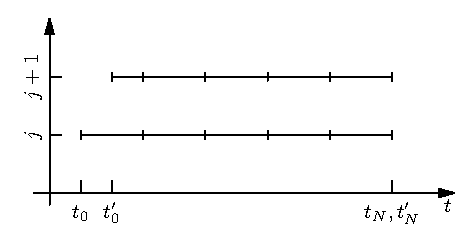
\includegraphics{mpc_subsampling.eps}}
        \subcaption{
            Reduction of the first sampling interval.
        }
        \label{fig.mpc_subsampling}
    \end{minipage}
    \hfill
    \begin{minipage}[t]{0.49\textwidth}
        \centering{%
        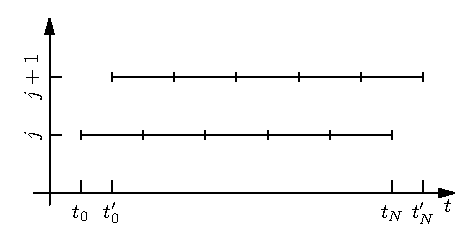
\includegraphics{mpc_nosubsampling.eps}}
        \subcaption{
            Shift of the whole preview horizon.
        }
        \label{fig.mpc_nosubsampling}
    \end{minipage}
    \caption[Sampling of the preview horizon.]{
        Sampling of the preview horizon on iterations $j$ and $j+1$
        with $T_c = T/2$ and $t_0^{\prime} = t_0 + T_c$.
    }
    \label{fig.mpc_sampling}
\end{figure}


The desired frequency of whole body motion control is higher than
$200~[\MT{Hz}]$, which corresponds to duration of a control interval $T_c$ in
the order of milliseconds \cite{Kuindersma2014icra, Herzog2015auro,
Saab2013tro}. Therefore, if an \ac{MPC} problem is resolved at such frequency,
in the form of \ac{MMPC} or as a part of two-stage control, it is necessary to
address discrepancy between $T$ and $T_c$. In this work we tried to employ two
heuristics for this purpose:
%
\begin{itemize}
    \item Reducing the first sampling interval $T_0$ by $T_c$ on each control
        iteration (\cref{fig.mpc_subsampling}). This can be interpreted as
        gradual removal of implicit \tn{move blocking} constraints, which
        impose that the control input is constant during $T_0$ (see also
        \cite{Cagienard2007jpc}).

    \item Shifting the whole preview horizon by $T_c$ on each control iteration
        (\cref{fig.mpc_nosubsampling}). The time instants at which constraints
        are imposed are shifted too. Thus, there is a problem of
        synchronization of changes in the model with the boundaries of sampling
        intervals as suggested in \cref{sec.discret_variation}. For example,
        consider a situation when a switch from a double to a single support is
        scheduled at time $t_0 + T$. If the constraint on the \ac{CoP} position
        is shifted from $t_0 + T$ with the preview horizon, there is a risk
        that the anticipated motion does not comply with this constraint at the
        instant of the switch. If we preserve constraints at such instants, the
        underlying optimization problem often becomes infeasible since the
        considered heuristic impairs recursive feasibility even in the case of
        time-invariant systems.
\end{itemize}
%
In either case, the structure of the \ac{MPC} problem changes significantly
from one control iteration to another due to changes in constraints. As a
result, the solutions obtained on subsequent iterations in general are not
equal on interval $[t_0^{\prime}, t_N]$, even in an ideal situation. In our
experience, this results in variations with period $T$ in solutions. Similar
behavior observed in \cite{Henze2014iros} is presumably caused by the same
reason. The second heuristic, however, yields much better results, which are
demonstrated later in \cref{ch.simulations}.


In conclusion of this discussion, it is necessary to emphasize that further
investigation of the sampling issue is needed, since neither of the proposed
heuristics is completely satisfactory.



%%%%%%%%%%%%%%%%%%%%%%%%%%%%%%%%%%%%%%%%%%%%%%%%%%%%%%%%%%%%%%%%%%%%%%%%%%%%%%%%
%%%%%%%%%%%%%%%%%%%%%%%%%%%%%%%%%%%%%%%%%%%%%%%%%%%%%%%%%%%%%%%%%%%%%%%%%%%%%%%%
%%%%%%%%%%%%%%%%%%%%%%%%%%%%%%%%%%%%%%%%%%%%%%%%%%%%%%%%%%%%%%%%%%%%%%%%%%%%%%%%
\section{Conclusion}

This chapter develops on the ideas and results of
\cref{ch.balance,ch.modeling}. We introduce \acf{MPC} as the tool for motion
anticipation and discretize approximate models constructed in
\cref{ch.modeling}, so that they can be used in \ac{MPC}. Then we construct
capturability constraints for these models to enforce capturability of
anticipated motion as suggested in \cref{ch.balance}. In addition to this, we
present our \acf{MMPC} approach to whole body motion control and anticipation
\cite{Sherikov2014humanoids, Sherikov2015humanoids}, and discuss some technical
details of \ac{MPC} implementation.
